\documentclass[12pt,a4paper]{article}
\usepackage[margin=1in]{geometry}
\usepackage[utf8]{inputenc}
\usepackage[polish]{babel}
\usepackage{polski}
\usepackage{amsfonts}
\usepackage{graphicx}
\usepackage{caption}
\begin{document}
    \begin{center}
        {\huge \textbf{access.analyser}}\\
        Karol Klimaszewski, Piotr Kowalski, Maciej Świderski
    \end{center}
    \section{Podsumowanie architektury}
        Aplikacja napisana jest w technologii ASP.NET Core 3.1 w stylu Model-View-Controller.
        Cała aplikacja będzie umieszczona w jednej warstwie instancji EC2.
        Zapewniona będzie wysoka dostępność przy użyciu ELB.\\
        Aplikacja korzysta z bazy danych PostgreSQL uruchomionej w ramach RDS do przechowywania danych użytkowników oraz danych otrzymanych z parsowania logów, a także z kubełków S3 do przechowywania logów w surowej postaci.\\
        Parsowanie logów wykonywanie jest za pomocą AWS Lambda w reakcji na upload logu do kubełka S3.
        Po zakończeniu parsowania otrzymane wartości umieszczane są w bazie danych, po czym mogą być przeanalizowane przez aplikację webową na żądanie użytkownika.\\
        Dodatkowo, jeśli jakiś użytkownik danego dnia doda więcej niż określona liczba logów, administrator dostanie powiadomienie email przy użyciu SNS.\\
        Poniżej umieszczone są diagramy architektury:
        \begin{center}
            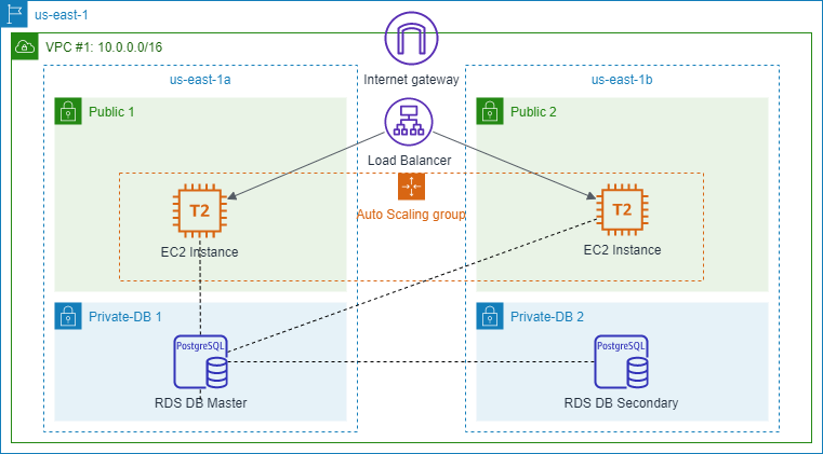
\includegraphics[scale=0.6]{d1.png}\captionof{figure}{Schemat architektury AWS}
            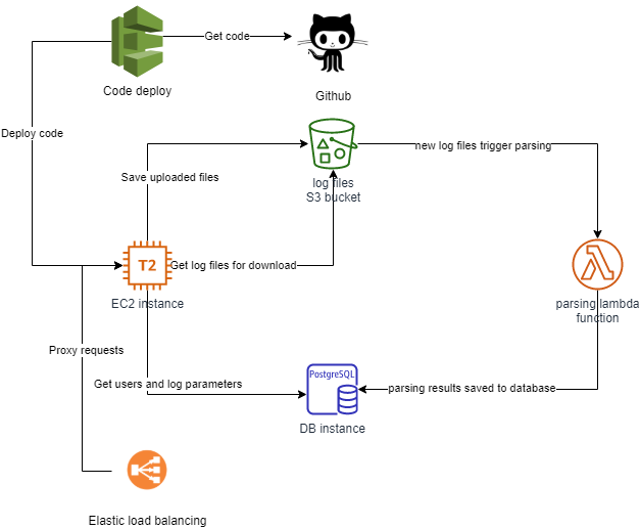
\includegraphics[scale=0.6]{d2.png}\captionof{figure}{Schemat integracji serwisów AWS}
        \end{center}
    \section{Użyte biblioteki i technologie}
        \begin{itemize}
            \item Biblioteki ASP.NET Core dostępne na licencji Apache License 2.0
            \item Npgsql do połączenia aplikacji z bazą danych - licencja PostgreSQL License
            \item AWS SDK do korzystania z S3 - licencja Apache License 2.0
            \item Biblioteki wykorzystywane do testów: xUnit oraz Moq, dostępne odpowiednio na licencji Apache 2.0 oraz BSD 3-Clause License
            \item Silnik bazy danych PostgreSQL dostępny na licencji PostgreSQL
        \end{itemize}
    \section{Instrukcja użytkownika}
        \subsection{Użytkownik niezalogowany}
            Niezalogowany użytkownik ma jedynie możliwość zalogowania się oraz założenia konta używając przycisków w prawym górnym roku strony.
            Do założenia konta wymagane jest podanie adresu email oraz hasła spełniającego wymagania.
        \subsection{Użytkownik zalogowany}
            Użytkownik zalogowany ma dostęp do menu zarządzania swoim kontem poprzez kliknięcie na swój adres email w prawym górnym roku strony.\\
            Na pasku górnym można przejść do zakładki ``Logs''.
            Daje ona możliwość wgrania, pobrania oraz usunięcia logu z bazy danych.
            Jeśli użytkownik nie ma statusu administratora, może zarządzać tylko logami wgranymi przez siebie.\\
            Na pasku górnym znajduje się również zakładka ``Analysis''.
            Pozwala ona na ustawienie zasad filtrowania oraz sortowania wpisów z logów przechowywanych w bazie danych.
            Użytkownik bez statusu administratora może przeglądać tylko wpisy z logów wgranych przez siebie.
        \subsection{Panel zarządzania użytkownikami}
            Jest to specjalny panel przeznaczony tylko dla użytkowników o statusie administratora.
            W tym panelu tacy użytkownicy mogą nadawać i odbierać użytkownikom status administratora, sprawdzać przypisanie użytkownikom tej roli, a także usuwać konta użytkowników.
    \section{Publiczne API}
        Aplikacja nie udostępnia żadnego publicznego API.
        Jedyny dostęp do aplikacji zapewniony jest przez stronę internetową.
    \section{Instrukcja postawienia na AWS}
    \section{Podsumowanie}
        Największym problemem w trakcie realizacji projektu okazały się ograniczenia konta AWS Educate.
        Niemożliwe okazało się testowanie programu na prywatnych kubełkach S3, a także współpraca w ramach jednego wspólnego VPC.
        Z tego samego powodu problematyczna okazała się także integracja z GitHubem.
        Również dlatego musieliśmy umieścić instancje EC2 w publicznych subnetach, co przy naszym układzie infrastruktury nie jest dobrym rozwiązaniem.
\end{document}